\section*{Цель работы}

\begin{enumerate}
    \item Исследование вольт-амперной характеристики (ВАХ) полупроводникового диода;
    \item Исследование работы однополупериодного выпрямителя;
    \item Исследование работы двухфазного двухполупериодного выпрямителя.
\end{enumerate}



\section*{Исходные данные}

Все исследования, проводимые в лабораторной работе, выполняются с диодом UMN1N 
и схемой двухфазного двухполупериодного выпрямителя согласно 16 варианту.



\section*{Снятие ВАХ полупроводникового диода}

\begin{figure}[htbp]
    \centering
    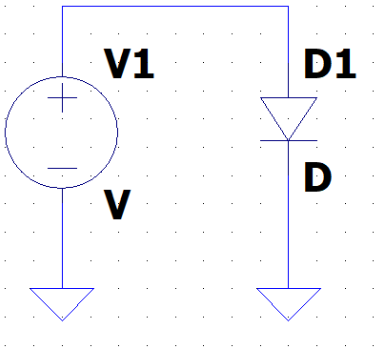
\includegraphics[width=0.3\linewidth]{figs/схема_иссл_вах.png}
    \caption{Схема для снятия ВАХ диода.}
    \label{fig:схемаисслвах}
\end{figure}

По ВАХ, которое было получено путем симуляции схемы на рисунке \ref{fig:схемаисслвах}, 
определим следующие параметры:
\begin{enumerate}
    \item Прямое статическое сопротивление диода.
    По рисунку \ref{fig:вах} с помощью курсоров в LTspice получаем, например, $U_\text{пр}=20.021622V$, $I_{\text{пр}}=11.579522A$
    и считаем
    $$
    R_\text{пр}=\frac{U_\text{пр}}{I_{\text{пр}}}=1.729054\Omega.
    $$
    \item Прямое дифференциальное сопротивление диода.
    По рисунку \ref{fig:вах} с помощью курсоров в LTspice получаем $\Delta U_\text{пр}=20.043243V$, $\Delta I_{\text{пр}}=12.186089A$
    и считаем
    $$
    R_\text{диф}=\frac{\Delta U_\text{пр}}{\Delta I_{\text{пр}}}=0.644764\Omega.
    $$
\end{enumerate}

\begin{figure}[htbp]
    \centering
    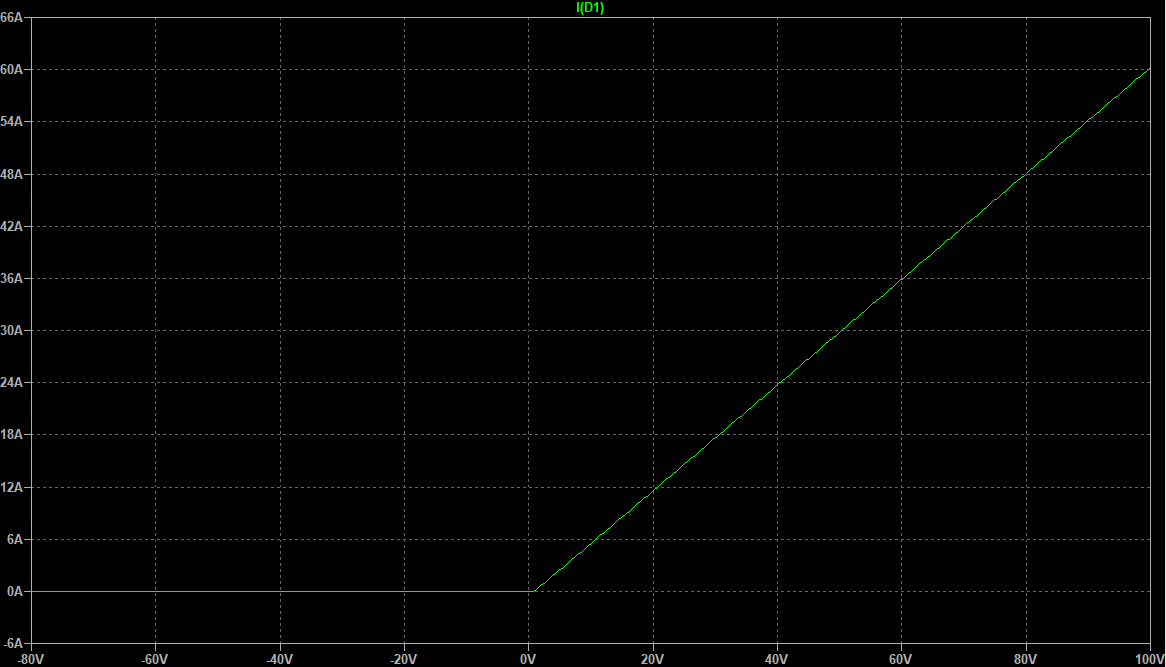
\includegraphics[width=1\linewidth]{figs/ВАХ_UMN1N.png}
    \caption{ВАХ диода UMN1N.}
    \label{fig:вах}
\end{figure}

Смотря на рисунок \ref{fig:вахzoomed} можно определить, что пороговое напряжение примерно $U_\text{пор}=640mV$.

\begin{figure}[htbp]
    \centering
    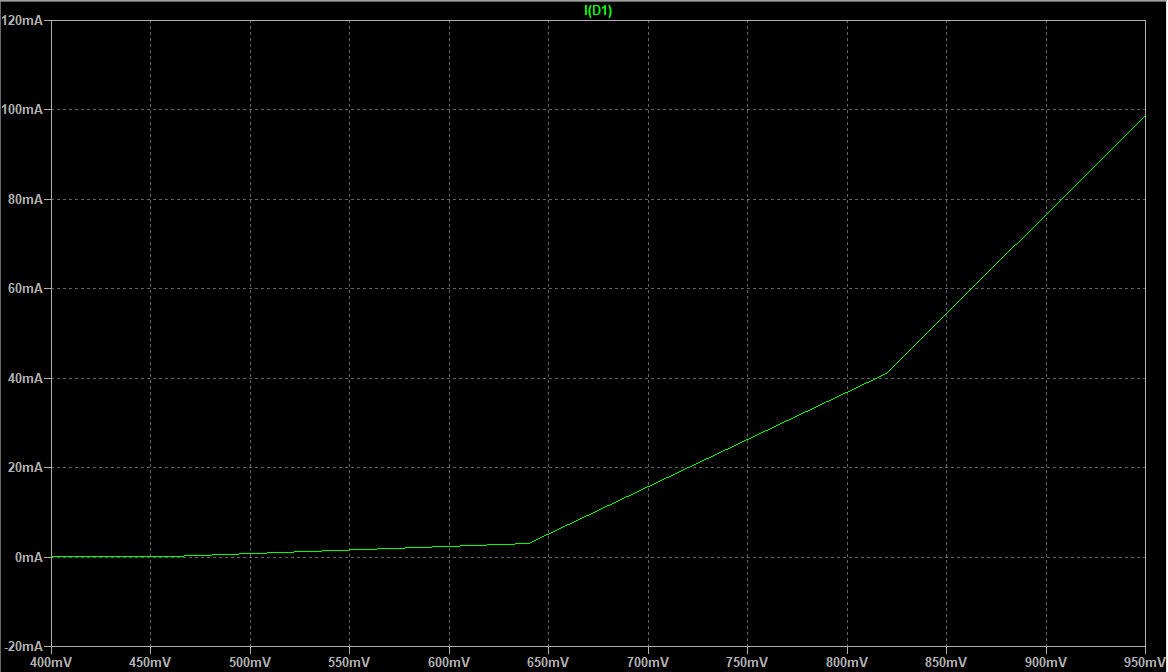
\includegraphics[width=1\linewidth]{figs/zoomed_ВАХ_UMN1N.png}
    \caption{ВАХ диода UMN1N увеличенная в начало зоны открытия.}
    \label{fig:вахzoomed}
\end{figure}

Напряжение пробоя у диода нет (параметр диода, который определяет наибольшее обратное напряжение, 
которое может быть приложено, не вызывая экспоненциального увеличения тока утечки в диоде),
так так какое бы напряжение не было приложено, сила тока убывала линейно (см. рисунок
\ref{fig:утечкатока}). Согласно технической документации максимальное обратное напряжение
составляет $80\text{В}$. 

\begin{figure}[htbp]
    \centering
    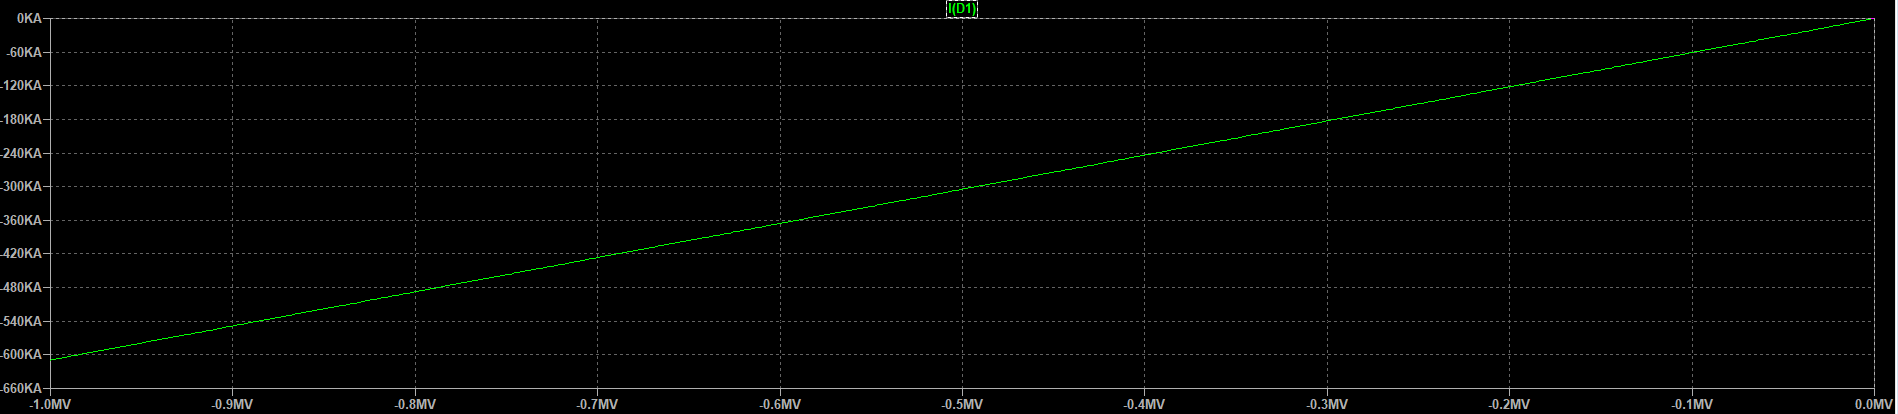
\includegraphics[width=1\linewidth]{figs/утечка_тока.png}
    \caption{Схема выпрямителя 16 варианта.}
    \label{fig:утечкатока}
\end{figure}



\section*{Исследование однополупериодного выпрямителя}

Используя схему на рисунке \ref{fig:схемаоднополупериодноговыпрямителя}, была получена 
осцилограмма однополупериодного выпрямителя (см. рисунок \ref{fig:осцилограмма}). 
Используя курсор в LTspice, находим максимальное напряжение на выходе, которое 
составляет около $U_{\text{вых}_{max}}\approx 9.4V$. 
Cредневыпрямленное значение напряжения на выходе выпрямителя, согласно формуле
$$
U_{\text{вых}_{\text{ср}}}=\frac{U_m}{\pi},
$$
равняется $U_{\text{вых}_{\text{ср}}}\approx 3V$.
Максимальное обратное напряжение на диоде составляет около $90\mu V$. Была смоделирована
ситуация пробоя диода, согласно технической документации напряжение пробоя составляет $-80V$,
что и подтверждается в симуляторе, где уже при $-82V$ отчетливо виден пробой. Для наглядности,
напряжение доходит до $90V$ на рисунке \ref{fig:осцилограммапробитая}.

\begin{figure}[htbp]
    \centering
    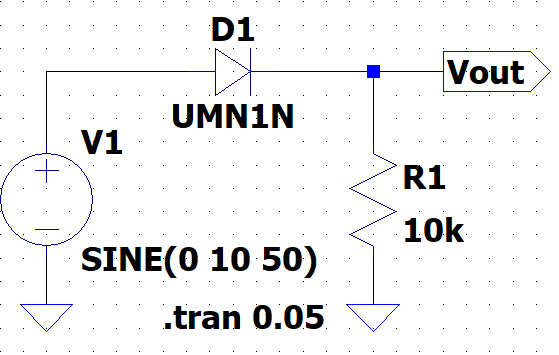
\includegraphics[width=0.5\linewidth]{figs/схема_однополупериодного_выпрямителя.png}
    \caption{Схема однополупериодного выпрямителя.}
    \label{fig:схемаоднополупериодноговыпрямителя}
\end{figure}

\begin{figure}[htbp]
    \centering
    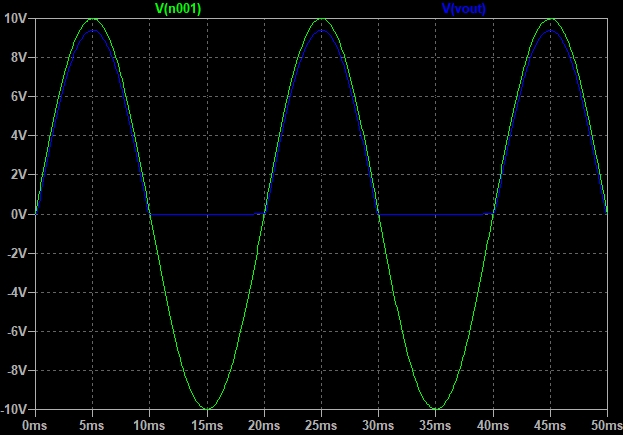
\includegraphics[width=0.8\linewidth]{figs/осцилограмма_выпрямителя.png}
    \caption{Осцилограмма однополупериодного выпрямителя.}
    \label{fig:осцилограмма}
\end{figure}

\begin{figure}[htbp]
    \centering
    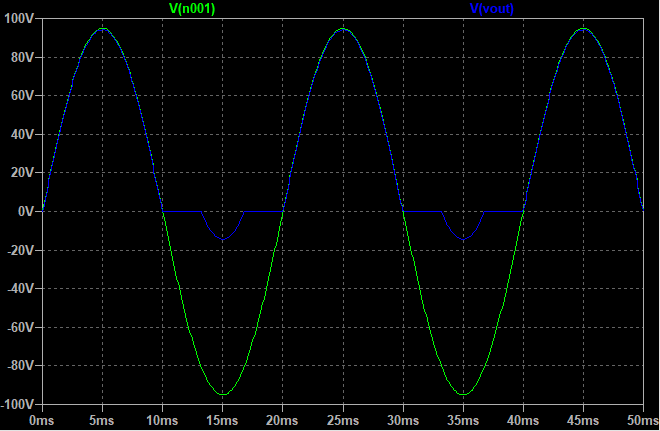
\includegraphics[width=0.8\linewidth]{figs/осцилограмма_пробитого_выпрямителя.png}
    \caption{Осцилограмма пробитого однополупериодного выпрямителя.}
    \label{fig:осцилограммапробитая}
\end{figure}


\section*{Исследование двухполупериодного выпрямителя}

Согласно моему варианту, была собрана схема как на рисунке \ref{fig:схемадвухполупериодноговыпрямителя},
С нее была снята осцилограмма (см. рисунок \ref{fig:осцдвухполупериодноговыпрямителя}).
Максимальное напряжение на выходе составляет $U_{\text{вых}_{max}}=9.39V$. Средневыпрямленное
значение напряжения согласно формуле
$$
U_{\text{вых}_{\text{ср}}}=\frac{2U_m}{\pi}
$$
равняется $U_{\text{вых}_{\text{ср}}}\approx 5.98V$. Максимальное обратное напряжение на диоде
нулю, так как минимальное напряжение наблюдаемое на выходе составляет около $70\mu V$, этот момент
можно видеть на рисунке \ref{fig:миннапряжениевыхода}. Был смоделирован пробой диода, его
можно увидеть на рисунке \ref{fig:пробойдвухполупериодноговыпрямителя}, пробой начинается, когда
источники напряжения в противофазе достигают $40V$ по модулю, их поля накладываются, и на один из
диодов приходят все $80V$, что и вызывает пробитие.

\begin{figure}[htbp]
    \centering
    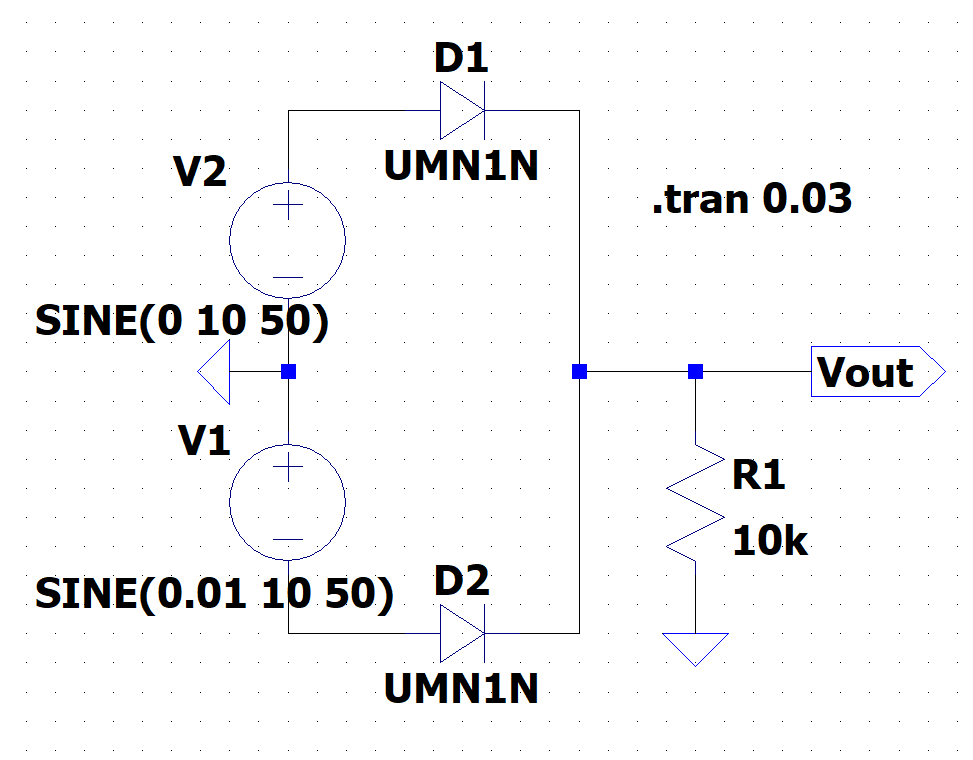
\includegraphics[width=0.6\linewidth]{figs/схема_двухполупериодного_выпрямителя.png}
    \caption{Схема двухполупериодного выпрямителя.}
    \label{fig:схемадвухполупериодноговыпрямителя}
\end{figure}

\begin{figure}[htbp]
    \centering
    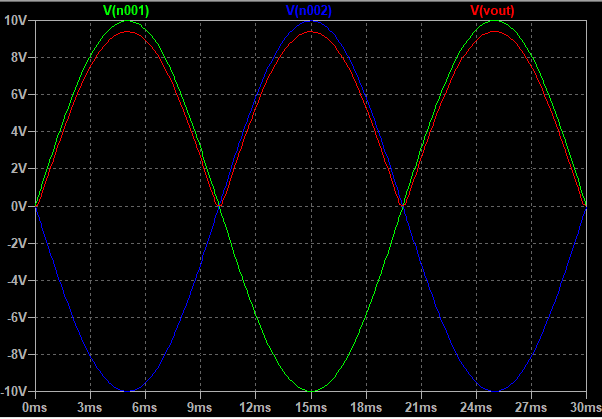
\includegraphics[width=0.8\linewidth]{figs/осц_двухполупериодного_выпрямителя.png}
    \caption{Осцилограмма двухполупериодного выпрямителя.}
    \label{fig:осцдвухполупериодноговыпрямителя}
\end{figure}

\begin{figure}[htbp]
    \centering
    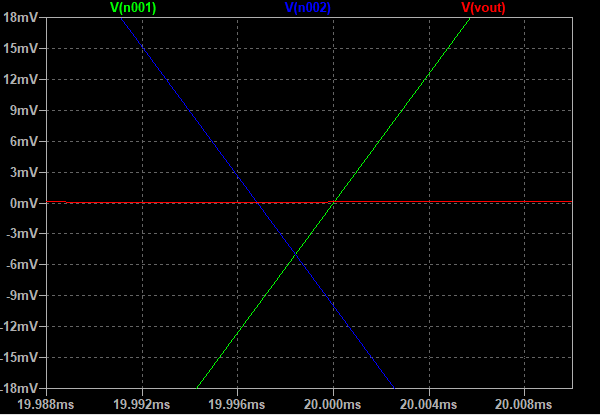
\includegraphics[width=0.8\linewidth]{figs/момент_мин_напряжения_на_диоде.png}
    \caption{Увеличеннная осфилограмма двухполупериодного выпрямителя на моменте минимального напряжения.}
    \label{fig:миннапряжениевыхода}
\end{figure}

\begin{figure}[htbp]
    \centering
    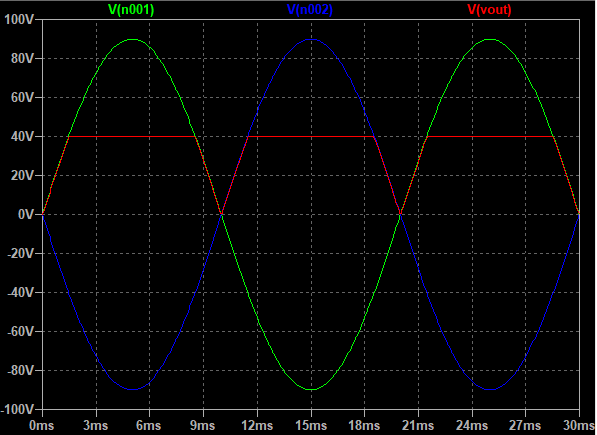
\includegraphics[width=0.8\linewidth]{figs/пробой_двухполупериодного_выпрямителя.png}
    \caption{Осцилограмма пробоя двухполупериодного выпрямителя.}
    \label{fig:пробойдвухполупериодноговыпрямителя}
\end{figure}



\subsection*{Исследование двухполупериодного выпрямителя с емкостным фильтром}

Согласно моему варианту была собрана схема как на рисунке \ref{fig:схемадвухполупериодноговыпрямителясфильтром},
емкость конденсатора была выбрана равной одному микро фарату, чтобы удовлетворять условию $\omega\cdot R_1\cdot C_1 < 1$.
Осцилограмму, снятую с данной схемы, можно увидеть на рисунке \ref{fig:осцдвухполупериодноговыпрямителясфильтром}.

\begin{figure}[htbp]
    \centering
    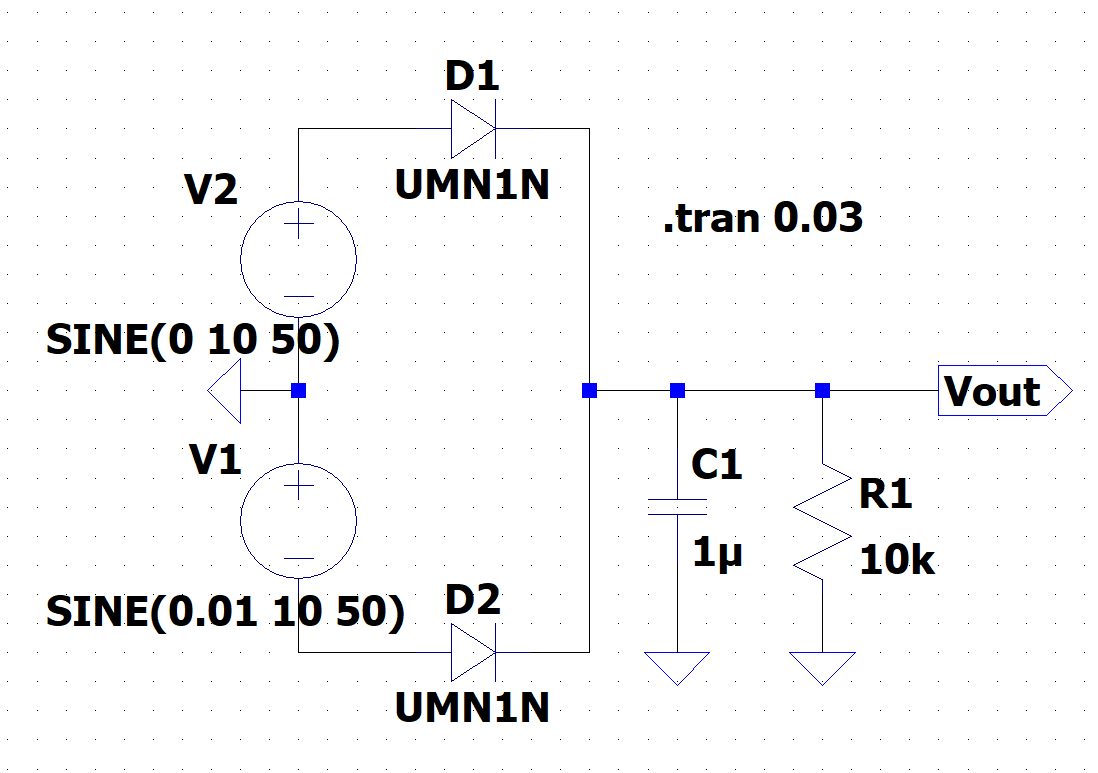
\includegraphics[width=0.8\linewidth]{figs/схема_двухполупериодного_выпрямителя_с_фильтром.png}
    \caption{Схема двухполупериодного выпрямителя с емкостным фильтром.}
    \label{fig:схемадвухполупериодноговыпрямителясфильтром}
\end{figure}

\begin{figure}[htbp]
    \centering
    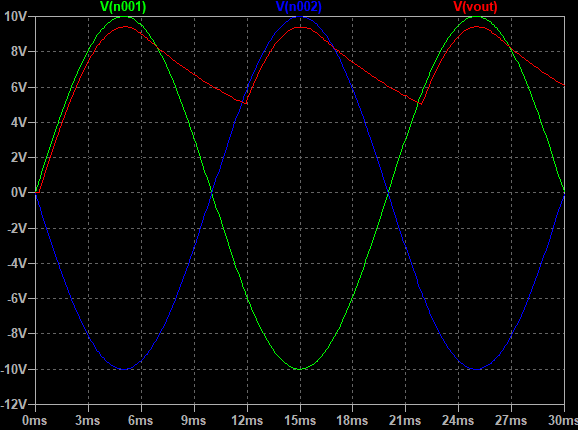
\includegraphics[width=0.8\linewidth]{figs/осц_двухполупериод_выпр_с_фильтром.png}
    \caption{Осцилограмма двухполупериодного выпрямителя с емкостным фильтром на $1\mu F$.}
    \label{fig:осцдвухполупериодноговыпрямителясфильтром}
\end{figure}

По осциллограмме определим максимальное и минимальное значения напряжения на выходе: 
$U_{\text{вых}_{max}}\approx 9.41V$, $U_{\text{вых}_{min}}\approx 5.02V$. Среднее значение выходного
сигнала, расчитанное LTspice, составляет $U_{\text{вых}_{\text{ср}}}= 7.188V$.
Найдем коэффициент пульсаций
$$
k=\frac{U_{\text{вых}_{max}} - U_{\text{вых}_{min}}}{U_{\text{вых}_{\text{ср}}}}=0.61.
$$
Если сравнивать его с коэффициентом $0.67$ у двухполупериодного выпрямителя, 
то можем сделать вывод, что схема с фильтром эффективнее. Если увеличить емкость конденсатора
до одного милли фарата (см. осцилограмму на рисунке \ref{fig:осцдвухполупериодноговыпрямителясфильтрувелемк}), то получиться выпрямить выходной сигнал, 
правда для этого понадобится время. У такой схемы после где-то 100мс почти пропадают пульсации 
(см. рисунок \ref{fig:осцдвухполупериодноговыпрямителясфильтрувелемк100}); но все-равно найдем
коэффициент пульсации на установившимся участке:
$U_{\text{вых}_{max}}\approx 9.25V$, 
$U_{\text{вых}_{min}}\approx 9.24\mu V$,
$U_{\text{вых}_{\text{ср}}}= 9.2497V$, коэффициент пульсаций $k=0.001$. Осцилограмма 
для прямоугольного сигнала
можно увидеть на рисунке \ref{fig:осцдвухполупериодноговыпрямителясфильтрувелемкпрямоуг}. 
Прямоугольные сигналы,
находясь в противофазе, почти всегда дают постоянное напряжение, что конденсатор с легкостью 
компенсирует и уже после 4мс
выходной сигнал остается постоянным и равным $9.41V$, что делает коэффициент 
пульсаций равным нулю.
Осцилограмму для пилообразного сигнала можно увидеть на рисунке 
\ref{fig:осцдвухполупериодноговыпрямителясфильтрпила}.
Найдем коэффициент пульсаций:
$U_{\text{вых}_{max}}\approx 9.40V$, 
$U_{\text{вых}_{min}}\approx 1.22\mu V$,
$U_{\text{вых}_{\text{ср}}}= 4.7846V$, тогда $k=1.71$, что делает схему наименее
эффективной.


\begin{figure}[htbp]
    \centering
    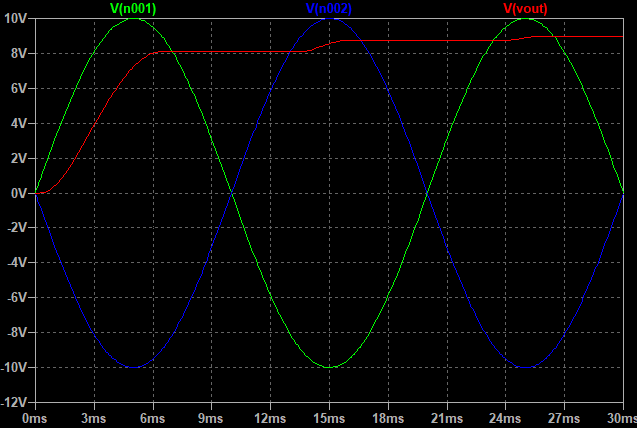
\includegraphics[width=0.8\linewidth]{figs/осц_двухпол_выпр_фильтр_увел_емк.png}
    \caption{Осцилограмма двухполупериодного выпрямителя с емкостным фильтром на $1\mu F$.}
    \label{fig:осцдвухполупериодноговыпрямителясфильтрувелемк}
\end{figure}

\begin{figure}[htbp]
    \centering
    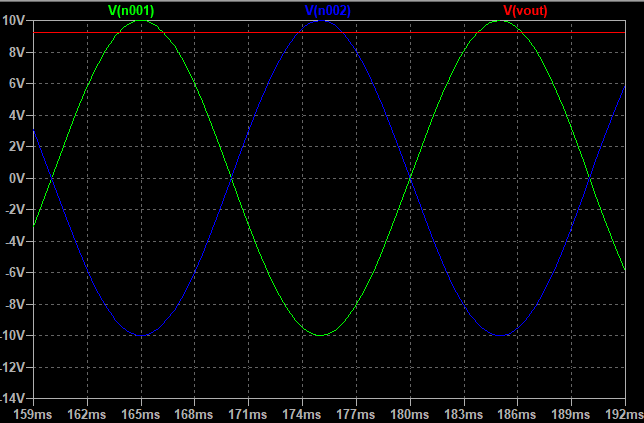
\includegraphics[width=0.8\linewidth]{figs/осц_двухпол_вып_фильтр_увл_емк_после_100.png}
    \caption{Осцилограмма двухполупериодного выпрямителя с фильтром увеличенной емкости до $1mF$ установившийся.}
    \label{fig:осцдвухполупериодноговыпрямителясфильтрувелемк100}
\end{figure}

\begin{figure}[htbp]
    \centering
    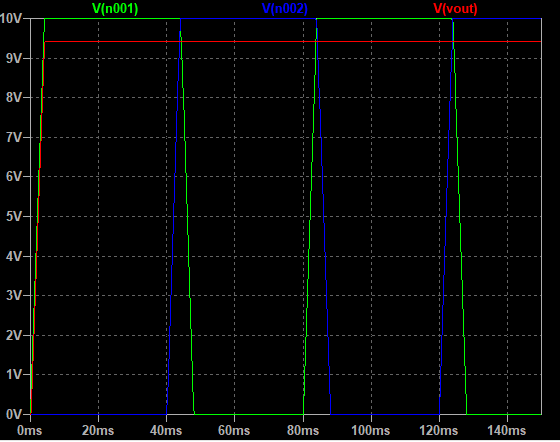
\includegraphics[width=0.8\linewidth]{figs/осц_двухпол_выпр_прямоуг.png}
    \caption{Осцилограмма двухполупериодного выпрямителя с емкостным фильтром на $1\mu F$ для прямоугольного сигнала.}
    \label{fig:осцдвухполупериодноговыпрямителясфильтрувелемкпрямоуг}
\end{figure}

\begin{figure}[htbp]
    \centering
    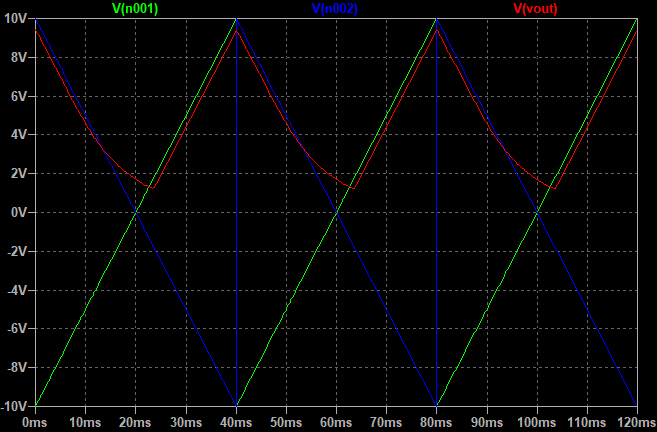
\includegraphics[width=0.8\linewidth]{figs/осц_двухпол_вып_фильтр_пила.png}
    \caption{Осцилограмма двухполупериодного выпрямителя с емкостным фильтром на $1\mu F$ для пилообразного сигнала.}
    \label{fig:осцдвухполупериодноговыпрямителясфильтрпила}
\end{figure}


\section*{Выводы}

В данной лабораторной работе было проведено исследование вольт-амперных характеристик
полупроводникового диода, работы однополупериодного и двухфазного 
двухполупериодного выпрямителей. Оценка качества выпрямителей для разлиных вариантов 
входного сигнала и емкости фильтра была получена и представлена в 
таблице \ref{tab:results}. По ней можно сделать вывод, что емкостный фильтр может очень серьездно
улучшить коэффициент пульсаций и добавить "разгон" схеме, но зато она 
становится более эффективной.

\begin{table}[htbp]
    \centering
    \begin{tabular}{|c|p{0.46\linewidth}|c|c|c|c|}
        \hline
        \textbf{№} & \textbf{Схема} & $\mathbf{U_{\text{вых}_{max}}},\ V$ & $\mathbf{U_{\text{вых}_{max}}},\ V$ & $\mathbf{U_{\text{вых}_{\text{ср}}}},\ V$ & $\mathbf{k}$\\
        \hline
        1 & Однополупериодный & 9.40 & - & 3.00 & 1.570\\
        \hline
        2 & Двухполупериодный & 9.39 & - & 5.98 & 0.670\\
        \hline
        3 & Двухполупериодный с фильтром на $1\mu F$ & 9.41 & 5.02 & 7.1880 & 0.610\\
        \hline
        4 & Двухполупериодный с фильтром на $1mF$ & 9.25 & 9.24 & 9.2497 & 0.001\\
        \hline
        5 & Двухполупериодный с фильтром на $1\mu F$ для прямоугольного сигнала & 9.41 & 9.41 & 9.41 & 0.000\\
        \hline
        6 & Двухполупериодный с фильтром на $1\mu F$ для пилообразного сигнала & 9.40 & 0.00 & 4.7846 & 1.71\\
        \hline
    \end{tabular}
    \caption{Таблица результатов}
    \label{tab:results}
\end{table}


